\documentclass[12pt]{iopart}

\usepackage{graphicx}
\graphicspath{{../fig/}}

\usepackage{url}
\usepackage{siunitx}
\usepackage{xr} % to cross-ref from review response
\externaldocument{./submission_02}
\usepackage{hyperref}
\hypersetup{hidelinks}
\usepackage{cleveref}

\begin{document}

\title{Supplemental Information: How unprecedented was the February 2021 Texas cold snap?}

\author{James Doss-Gollin$^1$, David J. Farnham$^2$, Upmanu Lall,$^{3,4}$ and Vijay Modi$^5$}
\address{$^1$ Department of Civil and Environmental Engineering, Rice University, Houston, TX, USA (ORCID 0000-0002-3428-2224)}
\address{$^2$ Department of Global Ecology, Carnegie Institution for Science, Stanford, CA, USA (ORCID 0000-0002-6690-4251)}
\address{$^3$ Columbia Water Center, Columbia University, New York, NY, USA (ORCID 0000-0003-0529-8128)}
\address{$^4$ Department of Earth and Environmental Engineering, Columbia University, New York, NY, USA}
\address{$^4$ Department of Mechanical Engineering, Columbia University, New York, NY, USA (ORCID 0000-0003-2513-0437)}
\ead{jdossgollin@rice.edu}
\vspace{10pt}

\submitto{\ERL}
\maketitle

\section{Supplemental Results}
\renewcommand{\thefigure}{S\arabic{figure}}
\setcounter{figure}{0}

\subsection{Historic Extreme Temperatures}

To complement \cref{fig:historic_era5}, we plot extreme cold temperatures using alternate data.
First, \cref{fig:historic_bk} shows historic events over the Continental United States.
The set of events is slightly different than that of \cref{fig:historic_era5}: the data set does not include the 2021 event, but does include the 1899 ``Great Blizzard.''
The 1899 event shows more intense and persistent cold than the other events in the dataset.
Next, \cref{fig:historic_tx} shows the same data as \cref{fig:historic_era5} but zooms in on Texas.
The 1989 (g-i) and 2021 (m-o) appear to be the most severe events in this data set, and the 1-day cold extremes in the 1989 event are more intense than in the February 2021 event, consistent with results in the main text.

\begin{figure}
  \centering
  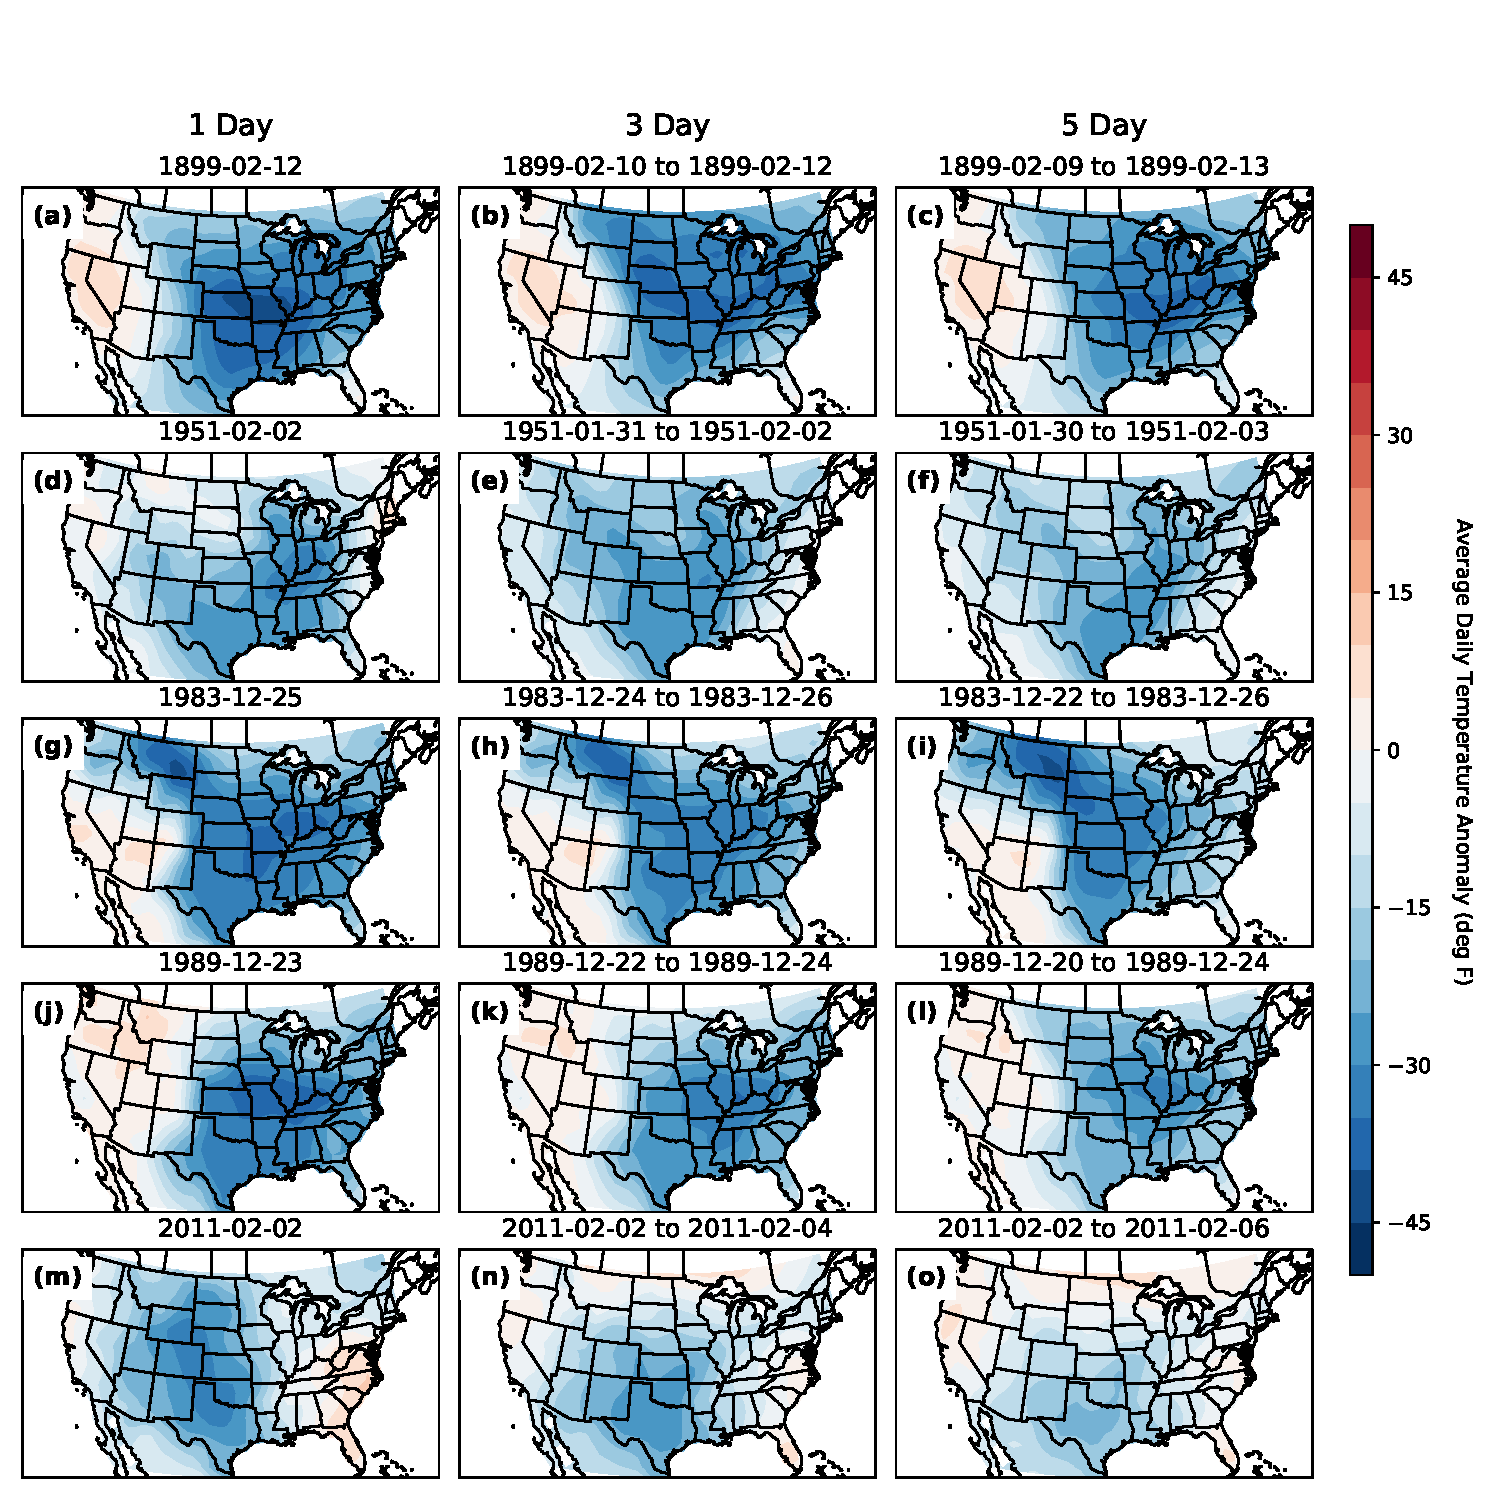
\includegraphics[width=\textwidth]{historic_events_bk.pdf}
  \caption{
    As \cref{fig:historic_bk} but the Berkely Earth temperature data is used.
    The dataset does not contain the 2021 event, but the ``Great Blizzard'' of February 1899 is included.
    Spatial patterns of cold from this dataset are qualitatively similar to Figure 1.
    The 1899 event emphasizes that the modern historical record does not yield a full sample from the full distribution of possible hazards.
  }\label{fig:historic_bk}
\end{figure}

\begin{figure}
  \centering
  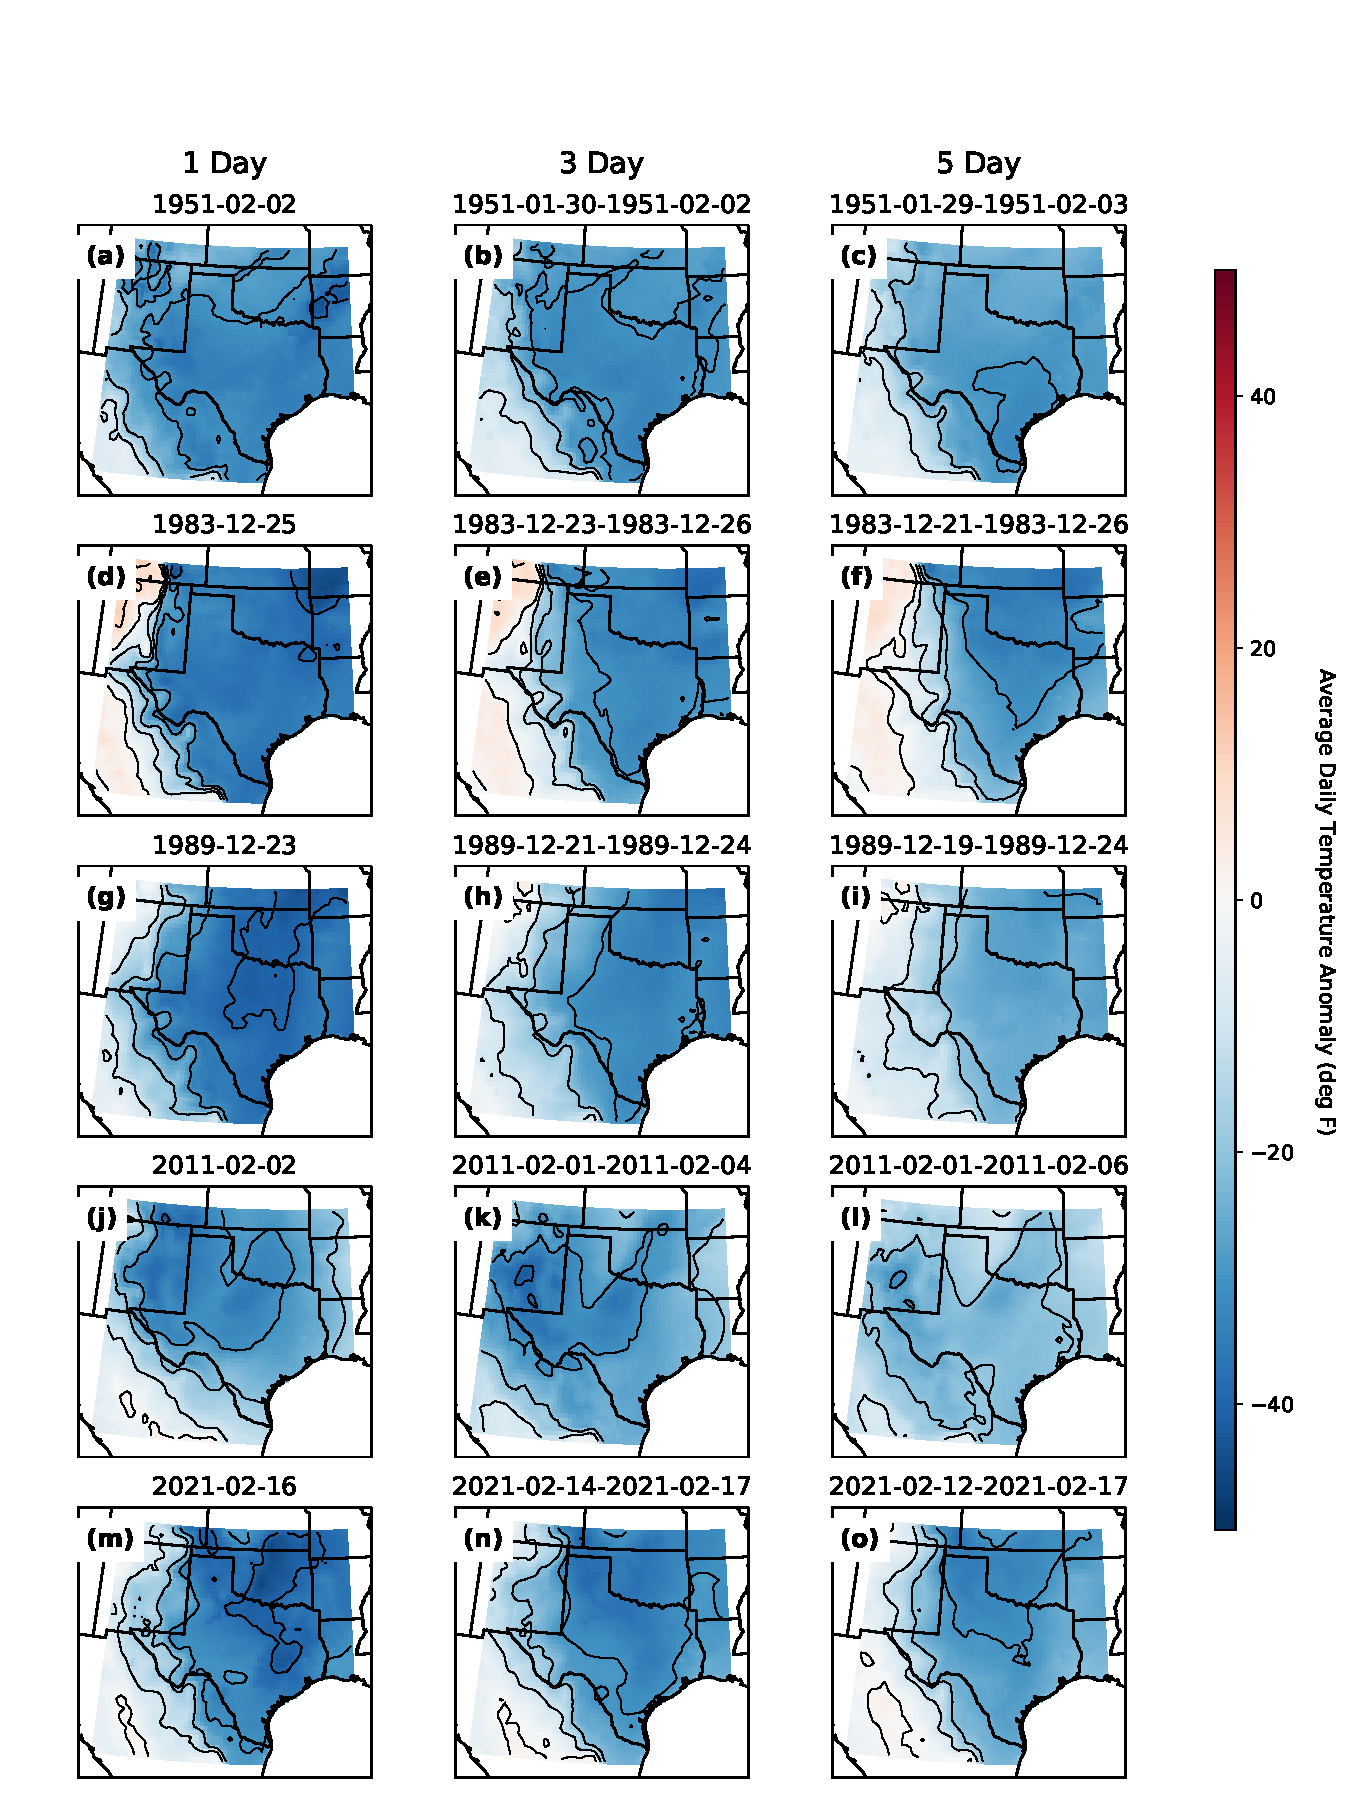
\includegraphics[width=\textwidth]{historic_events_era5_TX.pdf}
  \caption{
    As \cref{fig:historic_bk} but only Texas is shown.
  }\label{fig:historic_tx}
\end{figure}

\subsection{Spatially distributed temperature extremes}

To complement \cref{fig:local_era5}, we compute local return periods using station data from the GHCN \cite{Menne:2012hk}.
\Cref{fig:local_ghcnd} shows the return periods of the February 2021 cold snap for 1, 2, 3, and 4 day durations.
Only stations with at least 60 years of data are considered, and since the locations of these stations are not chosen at random, this does not constitute a representative sample of all points across Texas.
However, the spatial pattern matches that of \cref{fig:local_era5}, with a band of severe cold stretching from south-central to eastern Texas and in the Texas Panhandle.

\subsection{Inferred heating demand per capita}

To complement our analysis of inferred heating demand per capita, we consider how results change as a function of two modeling decisions.
First, we consider what happens if the spatial field demand for heating is aggregated using grid cell area rather than population density.
Next, we compute return periods using an estimator based on the method of $L$-moments.
Although $L$-moment estimators for the generalized extreme value distribution are not unbiased, they are popular in the statistical hydrology literature for their stability \cite{hosking_gev:1985,martins_gev:2001,morrison_gev:2002}.

We draw two conclusions from these plots.
First, the 2021 event appears more severe if grid cells are weighted by population density (\cref{fig:idf_weighted,fig:idf_lmoments_weighted}) than if they are weighted only by area \cref{fig:idf_unweighted,fig:idf_lmoments_unweighted}).
This is consistent with our observation of a correspondence between the most extreme temperatures in February 2021 and population density (\cref{fig:local_era5}).
By contrast, the 2011 event appears more extreme when grid cells are weighted by area, which is consistent with \cref{fig:historic_tx,fig:historic_era5,fig:historic_bk} showing the coldest temperatures in relatively less populated West Texas.
Second, the $L$-moment estimators (\cref{fig:idf_lmoments_weighted,fig:idf_lmoments_unweighted}) assign a lower return period to the 1989 and 2021 events than the maximum likelihood estimators (\cref{fig:idf_unweighted,fig:idf_weighted}).

To provide some context for our inferred demand for heating metric, \cref{fig:hdd_ts} plots its time series during the peak of the February 2021 cold snap.
This reveals a rise from approximately \SI{10}{\degree F} to nearly \SI{60}{\degree F} during the peak of the February 2021 cold snap.

\begin{figure}
  \centering
  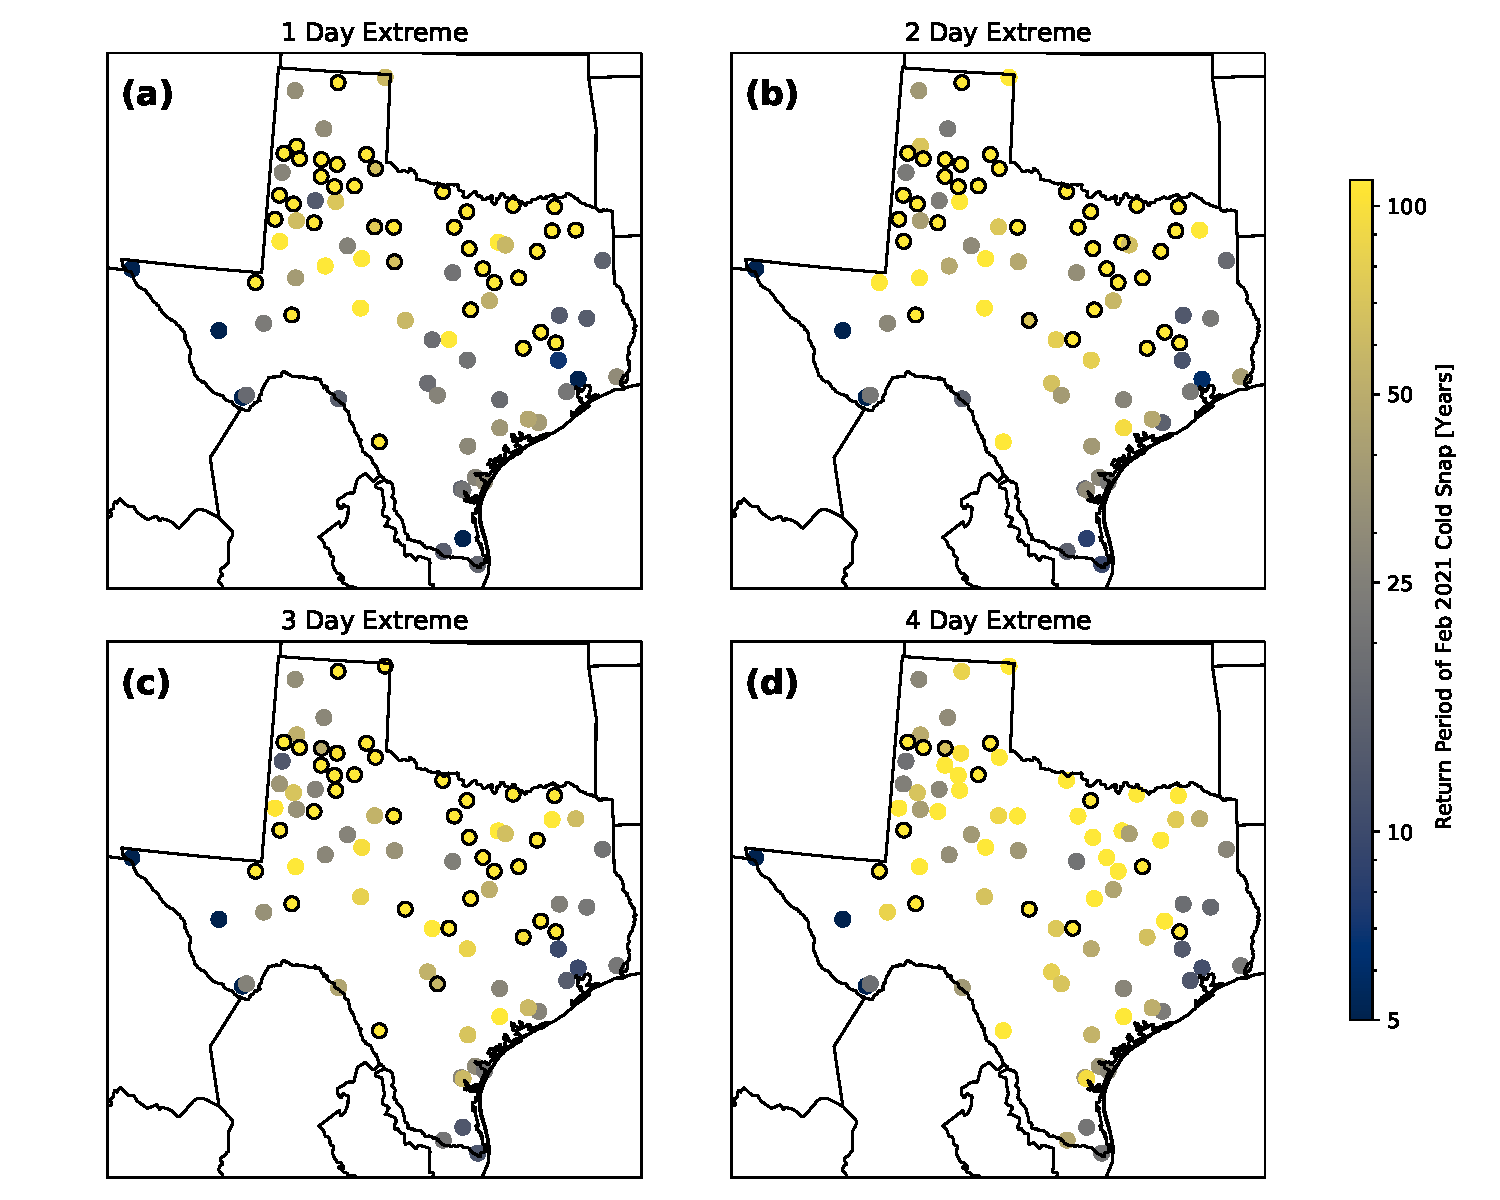
\includegraphics[width=\textwidth]{local_rt_ghcnd.pdf}
  \caption{
    As \cref{fig:local_era5} but return periods are calculated using station data from the GHCN data set \cite{Menne:2012hk}.
    Black circles indicate that a station exceeded its own record for a particular duration.
  }\label{fig:local_ghcnd}
\end{figure}

\begin{figure}
  \centering
  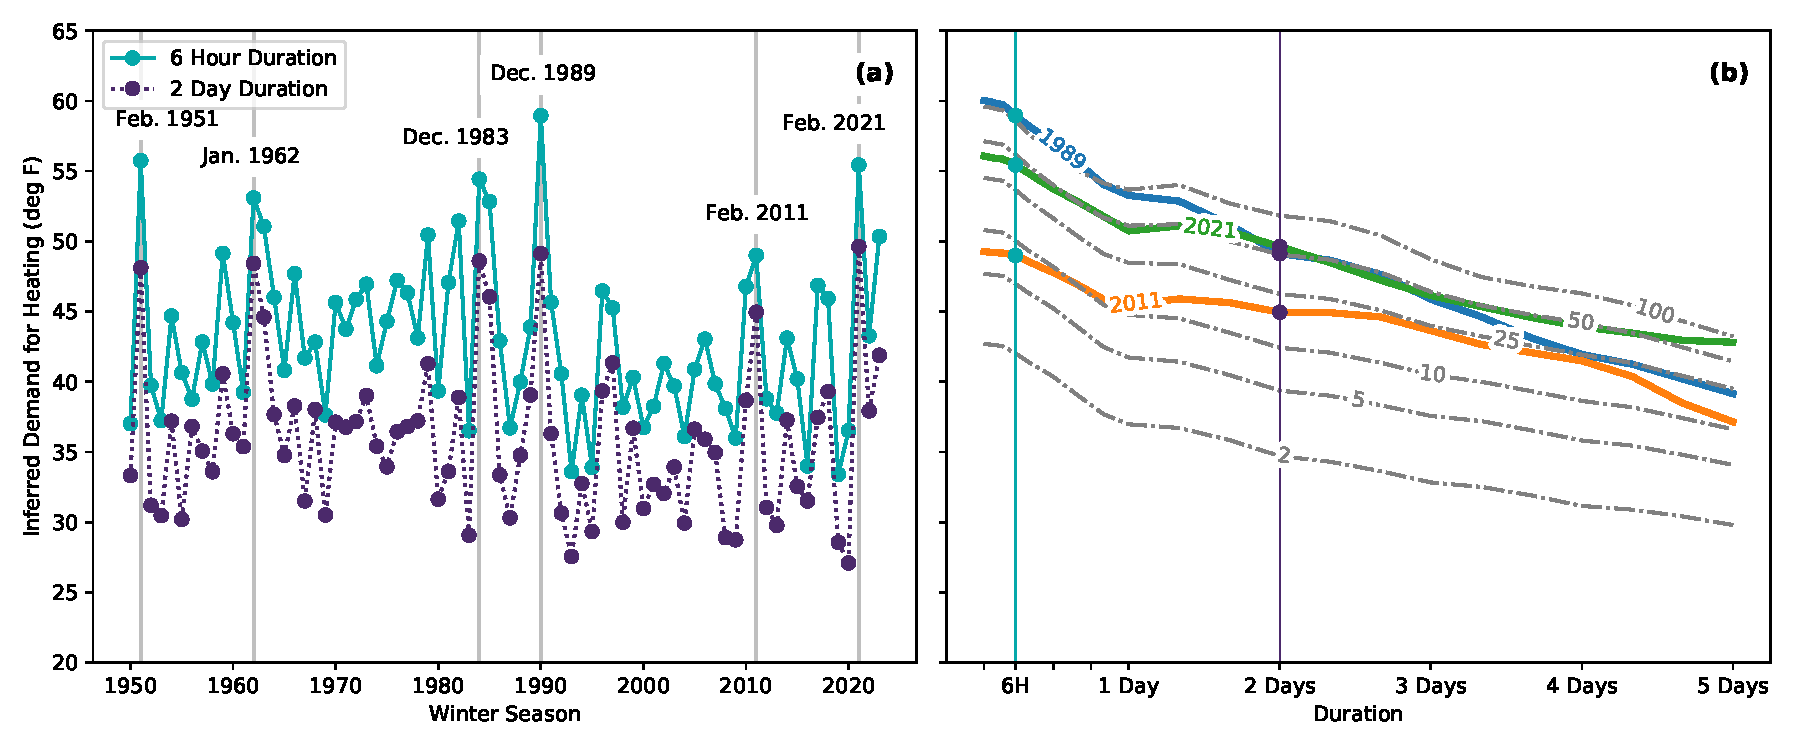
\includegraphics[width=\textwidth]{ERCOT_HDD_IDF_MLE_unweighted.pdf}
  \caption{
    As \cref{fig:idf_unweighted} but grid cells are weighted by area $A=\cos(\phi)$ where $\phi$ is latitude.
  }\label{fig:idf_unweighted}
\end{figure}

\begin{figure}
  \centering
  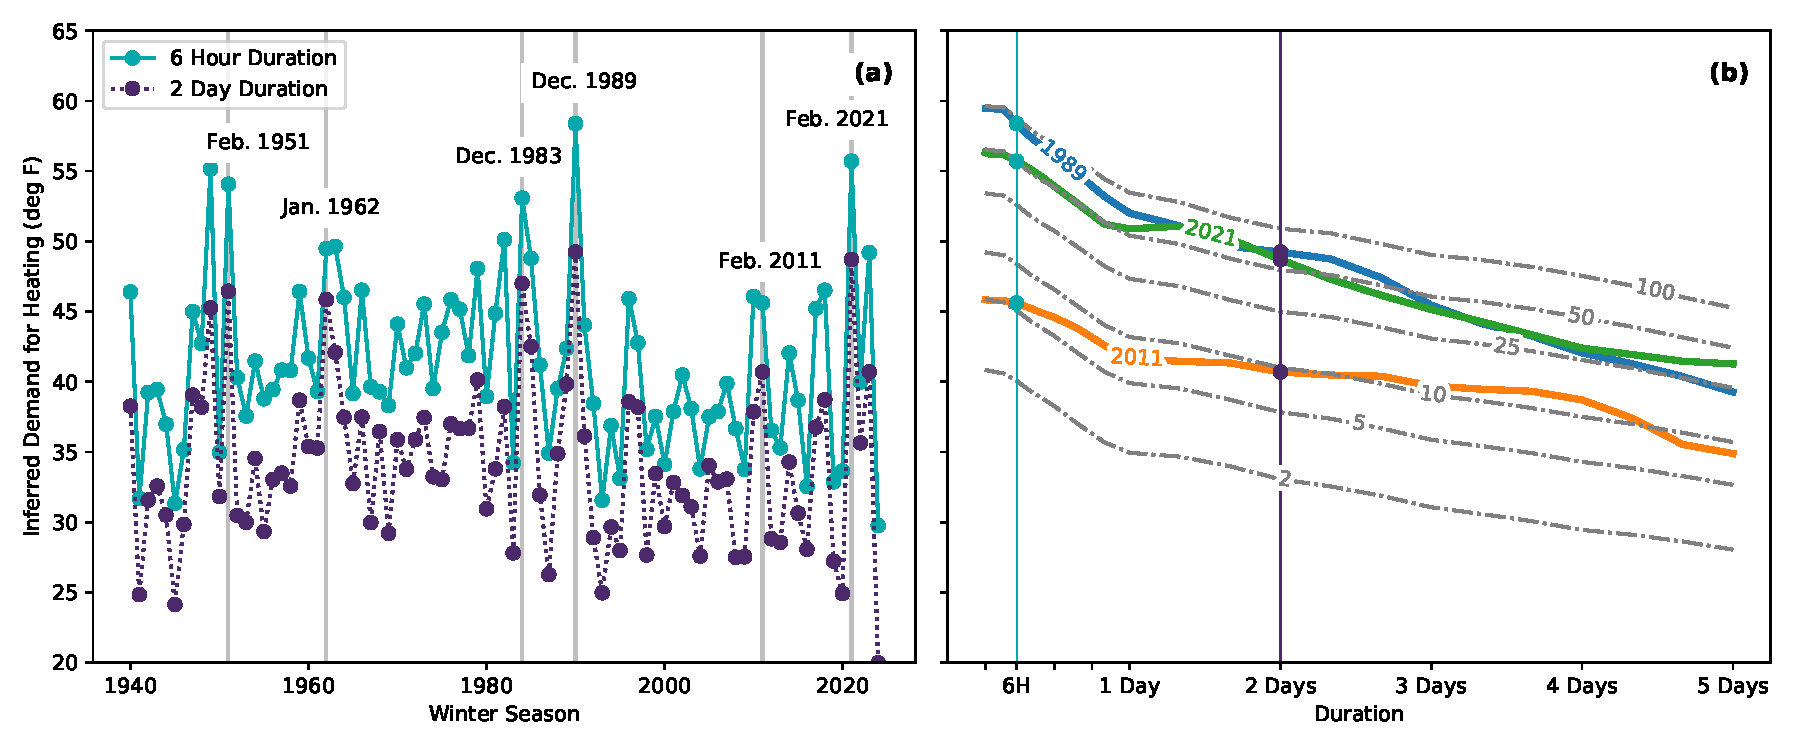
\includegraphics[width=\textwidth]{ERCOT_HDD_IDF_plotpos_popweighted.pdf}
  \caption{
    As \cref{fig:idf_unweighted} but return periods are calculated using the $L$-moments estimator.
  }\label{fig:idf_lmoments_weighted}
\end{figure}

\begin{figure}
  \centering
  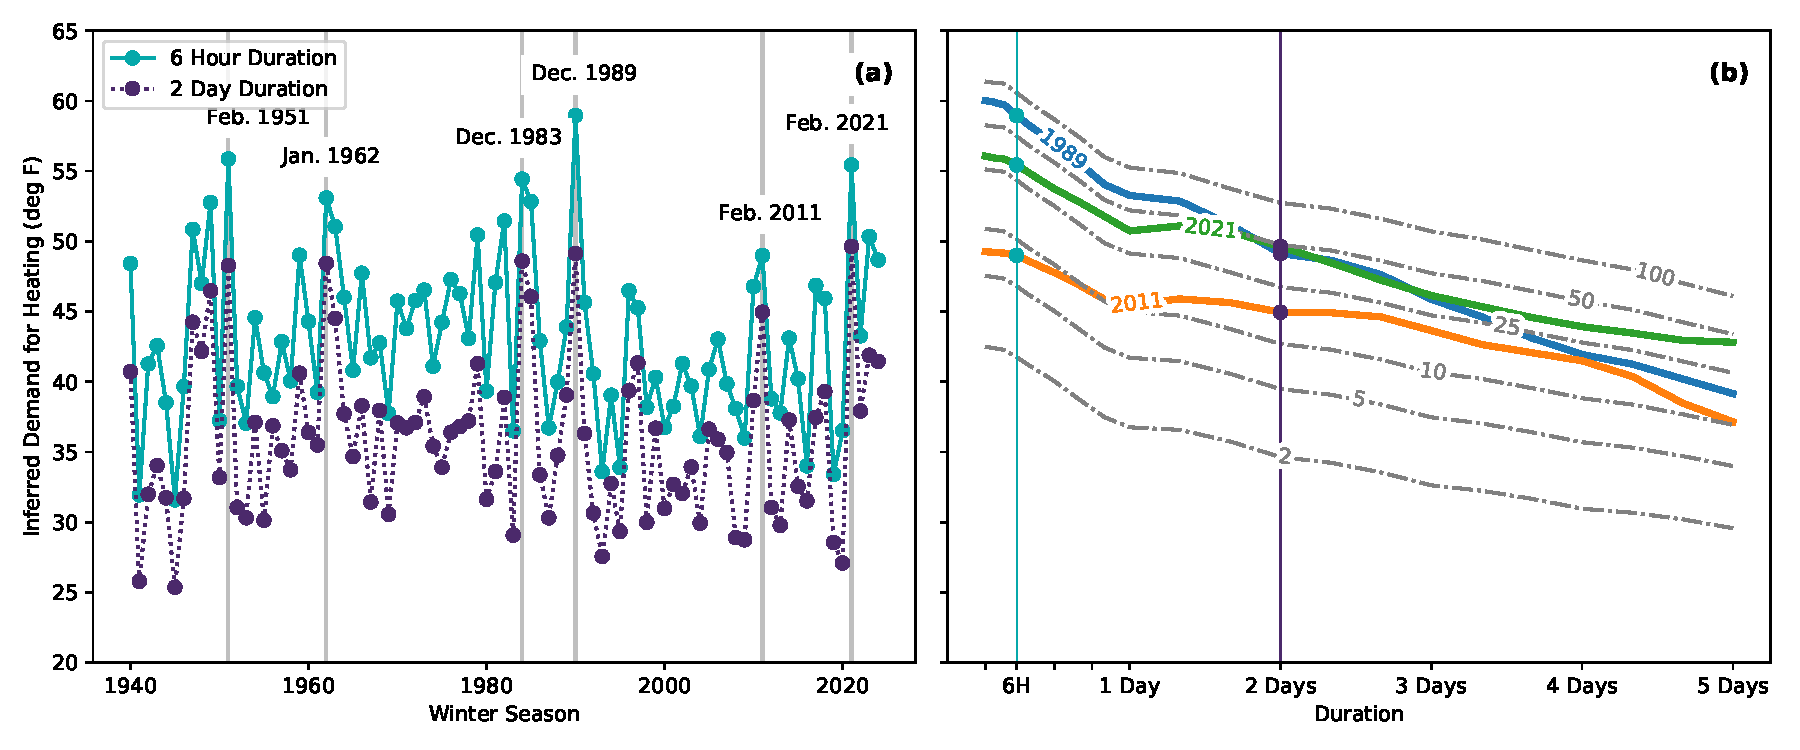
\includegraphics[width=\textwidth]{ERCOT_HDD_IDF_plotpos_unweighted.pdf}
  \caption{
    As \cref{fig:idf_unweighted} but return periods are calculated using the $L$-moments estimator.
  }\label{fig:idf_lmoments_unweighted}
\end{figure}

\begin{figure}
  \centering
  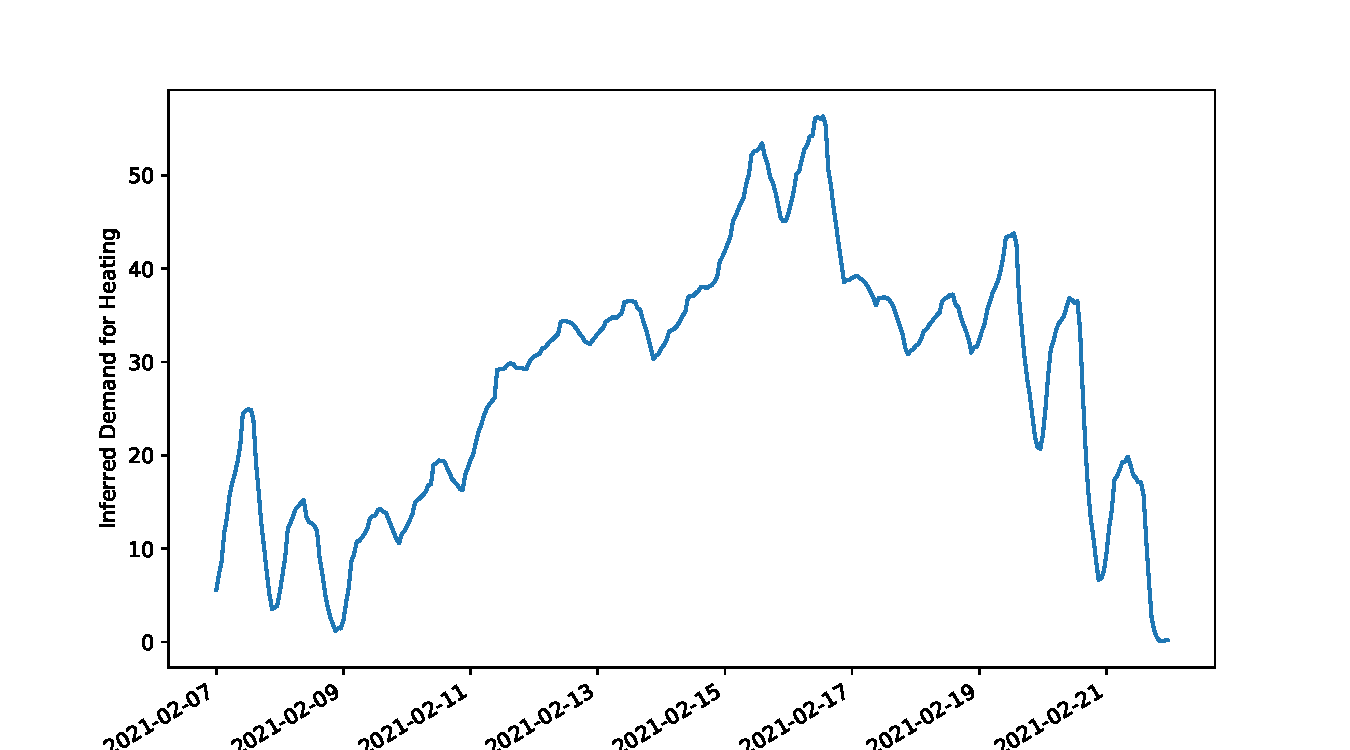
\includegraphics[width=\textwidth]{HDD_pop_weighted_ts.pdf}
  \caption{
    A time series of inferred heating demand per capita over the Texas Interconnection during the February 2021 cold snap.
  }\label{fig:hdd_ts}
\end{figure}

\begin{figure}
  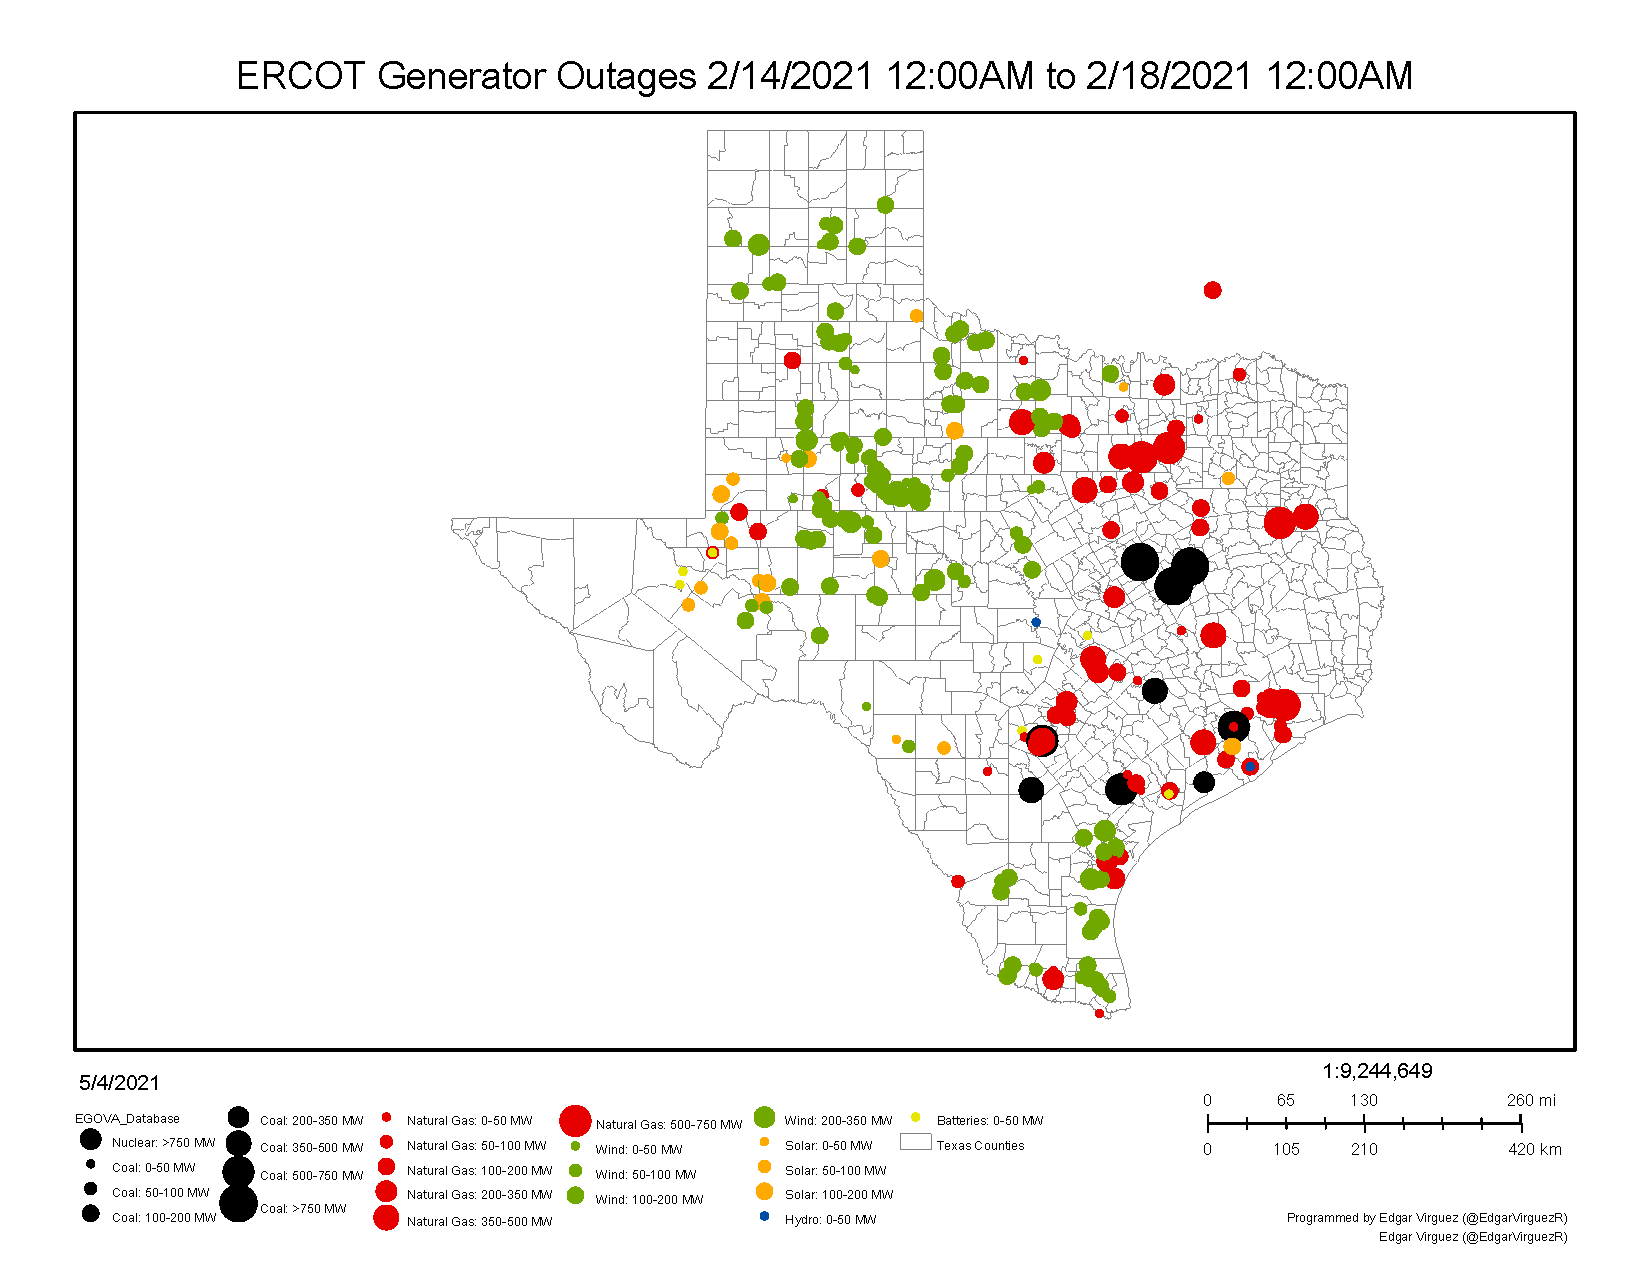
\includegraphics[width=\textwidth]{EGOVA.pdf}
  \caption{
    ERCOT generator outages from 12:00AM on 14 February 2021 to 12:00AM on 18 February 2021.
    Map produced using ERCOT's Generator Outage/Derate Visualization App (EGOVA) available at \url{https://bit.ly/EGOVA}.
    Dot sizes describe the capacity reduction for each outage or derate event, which may not be the same as the difference between the power produced and what ERCOT anticipated, particularly for intermittent resources \cite{ercotpublic_outagesv2:2021}.
  }\label{fig:egova}
\end{figure}

\end{document}
